\section{Finger}

\subsection{Kleberdosierung}
	
	\subsubsection{DAS MUSS IN METHODE!}
	Am Anfang wurde die Klebermenge mithilfe einer Pinzette dosiert. Hierfür wurde das HFE zuallererst in ein Bad gegeben, welches auf -140??°C gekühlt wurde. Bei diesen Temperaturen verdampft das HFE nicht mehr. außerdem wird das HFE Dickflüssig. Mit einer Pinzette wird dann nun die benötigte Menge auf die Fingerspitze aufgetragen. Jedoch kann die genaue Menge auf dem Finger nur qualitativ abgeschätzt werden.
	
	Um die optimale Klebermenge quantitativ zu bestimmen, wurde das HFE mit Hilfe einer Pipette (MARKE) Pipettiert. 
	
\subsection{Temperaturtest}
\subsection{Ablöserichtung}


\section{PDMS}

	\begin{figure}[h]
		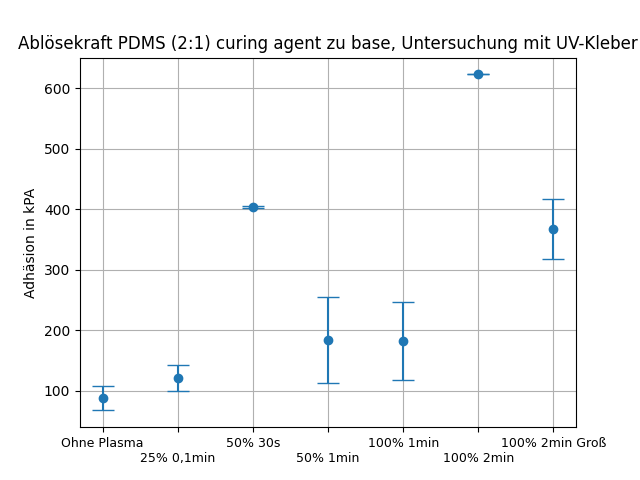
\includegraphics[width=14cm]{test}
		\caption{PDMS 2:1 vergleich bei verschiedenen Plasmacuring stärken und längen.}
	\end{figure}

\section{Lipide}


\begin{figure}[h]
	\begin{tabular}{|c|c|c|c|c|}
		\hline
		Lipide & 4-Methyl Pentene & 3-Methyl Pentene & 1-Pentene & Isopentane \\
		\hline
		EGG-PC & Ja & Geht & Nein & Nein \\
		\hline
		DOPC & ? & Nein & Nein & Geht \\
		\hline
	\end{tabular}
	\begin{tabular}{|c|c|c|c|}
		\hline
		Lipide &  1-Propanol & Pentane & Ethanol \\
		\hline
		EGG-PC & Ja & Ja & ? \\
		\hline
		DOPC & Ja & Nein & Ja \\
		\hline
	\end{tabular}
	\caption{Getestete Lipide und Lösungsmittel unter Raumtemperaturen}
\end{figure}

